\begin{frame}{Les industries éditoriales et
littéraires}
 Une IA qui va intégrer par contre des outils d'édition :
\begin{itemize}
    \item révision de texte
    \item gestion des plannings
    \item communication
    \item Globalement, une industrie qui apprécie une forme d'artisanat et qui se montre assez réfractaire.
\end{itemize}


Cas particulier : illustrateurs.
\end{frame}

\begin{frame}{Cas n°1 : Mathis et la forêt des possibles}
\begin{block}{}
    \centering
    
\includegraphics[width=0.60\textwidth]{04_Axe1_IAG/Images/mathis-Foret.png}
\end{block}
\begin{itemize}
    \item Collaboration entre les PUR et la maison d'édition Locus Solus
    \item Jiri Benovsky est spécialiste en métaphysique, en philosophie de l’esprit et en esthétique. Pas illustrateur.
    \item Son premier album jeunesse, réalisé par IA.
\end{itemize}

\end{frame}

\begin{frame}{Un bon prompteur peut-il remplacer un illustrateur ?}
\begin{block}{}
\textrightarrow{} Qu'est-ce que c'est que le geste de création ?
    \textrightarrow{} Vieux débat sur les conditions et les compétences pour mériter le statut d'artiste.
\end{block}
\centering
    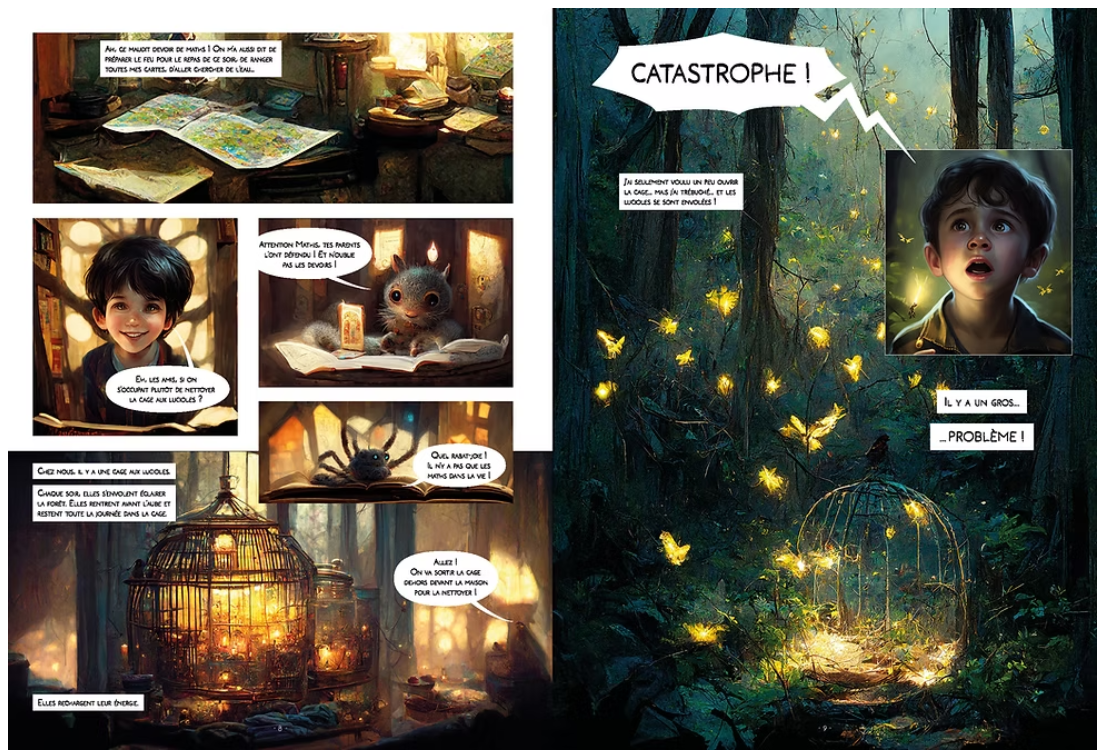
\includegraphics[width=0.60\textwidth]{04_Axe1_IAG/Images/mathisEtLaForetDesPossibles.png}
\end{frame}

\begin{frame}{La problématique des données et des modèles entraînés}
On a toujours utilisé des outils pour nous aider dans notre travais mais est-ce qu'une IA est un outil comme un autre ? \\
Exemple: des IA entraînées sur des oeuvres protégées par le droit d'auteur.\\
\vspace{3mm}
\begin{block}{}
    \centering
    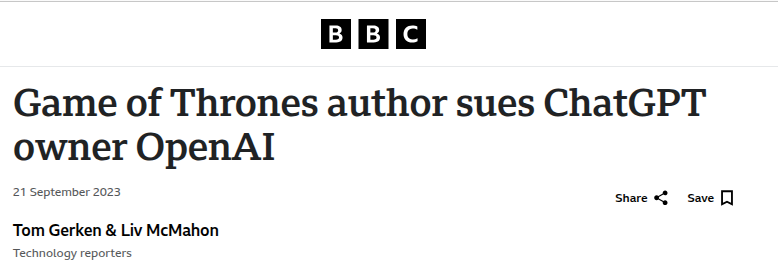
\includegraphics[width=0.70\textwidth]{04_Axe1_IAG/Images/author_suing_gpt.png}
\end{block}

\textrightarrow{} Crainte des créateur.rices de l'accaparement de la propriété intellectuelle, baffouée par les modèles.
\end{frame}

\begin{frame}{Constituer et entraîner un VML : un geste technique, un geste auctorial ?}
\begin{itemize}
    \item Constituer son modèle et l'entraîner : la réalité des pionniers
    \item Le développement vers des outils grand public menace de faire disparaître la technicité
\end{itemize}
Selon Frédéric Maupomé, "\textit{Les IA n’inventent rien : il leur faut plagier la création humaine, en s’inspirant de centaines de millions d’images et métadonnées aspirées automatiquement sur internet.}"

\end{frame}

\begin{frame}{Un droit à l'\textit{opt-out} peu efficace}

\textbf{\textit{opt-out}}= désigne la possibilité pour une personne, une organisation ou un créateur de refuser que ses données, œuvres ou contenus soient utilisés pour l’entraînement, l’évaluation ou le fonctionnement d’un modèle d’IA.\\
\vspace{5mm}

\centering
{\small

\textit{Un calvaire ! C'est image par image, il faut prouver qu'on est l'ayant droit, recommencer parfois à chaque copie présente dans la base, (ex. Have i been trained). Et recommencer pour chaque base... Sans preuve d'effet (et l'opt-out n'est pas rétroactif), si on est dans la base,c'est trop tard. Les restrictions mises en place par les entreprise d'IA (par exemple on ne peut pas demander d'image dans le style de Steve mc curry à stable diffusion, il y a un filtre sur son nom) sont facilement contournées (par exemple en écrivant mal les noms).}}\\
\textbf{ Positionnement de la Ligue des auteurs professionnels}
\end{frame}

\begin{frame}{Atelier: Du programme au prompt : comprendre les stratégies de génération de récits à l’heure des LLM}
\centering
    
\includegraphics[width=4cm]{04_Axe1_IAG/Images/atelier-prompt.png}
\end{frame}

\begin{frame}{Au-delà des industries culturelles et créatives...}
\begin{itemize}
    \item Des enjeux éthiques : entraînement des données et \textit{digital labour}
    \item Des enjeux politiques : nouveaux monopoles, vectofascisme
    \item Des enjeux écologiques : coût d'entraînement des modèles (calcul, stockage)
\end{itemize}
    
\end{frame}

\begin{frame}{L'IA Act: un premier pas en faveur de la régulation}
   \begin{columns}[T,onlytextwidth]
\column{0.50\linewidth}
\small
\textit{Puisqu’il sera impossible de garantir l’absence de discrimination sous tous les angles, des choix seront nécessaires, et des seuils de tolérance devront être définis. Se pose alors la question : quel est le niveau acceptable d’erreurs et de quel type d’erreurs parle-t-on ? Ce qui revient à se demander : quel est le niveau « acceptable » de risque de discrimination ?}\\ 
\textbf{Mélanie Gornet et Winston Maxwell, "\textit{Intelligence artificielle: normes techniques et droits fondamentaux, un mélange risqué}", The Conversation, 2022.}
\column{0.50\linewidth}
\centering
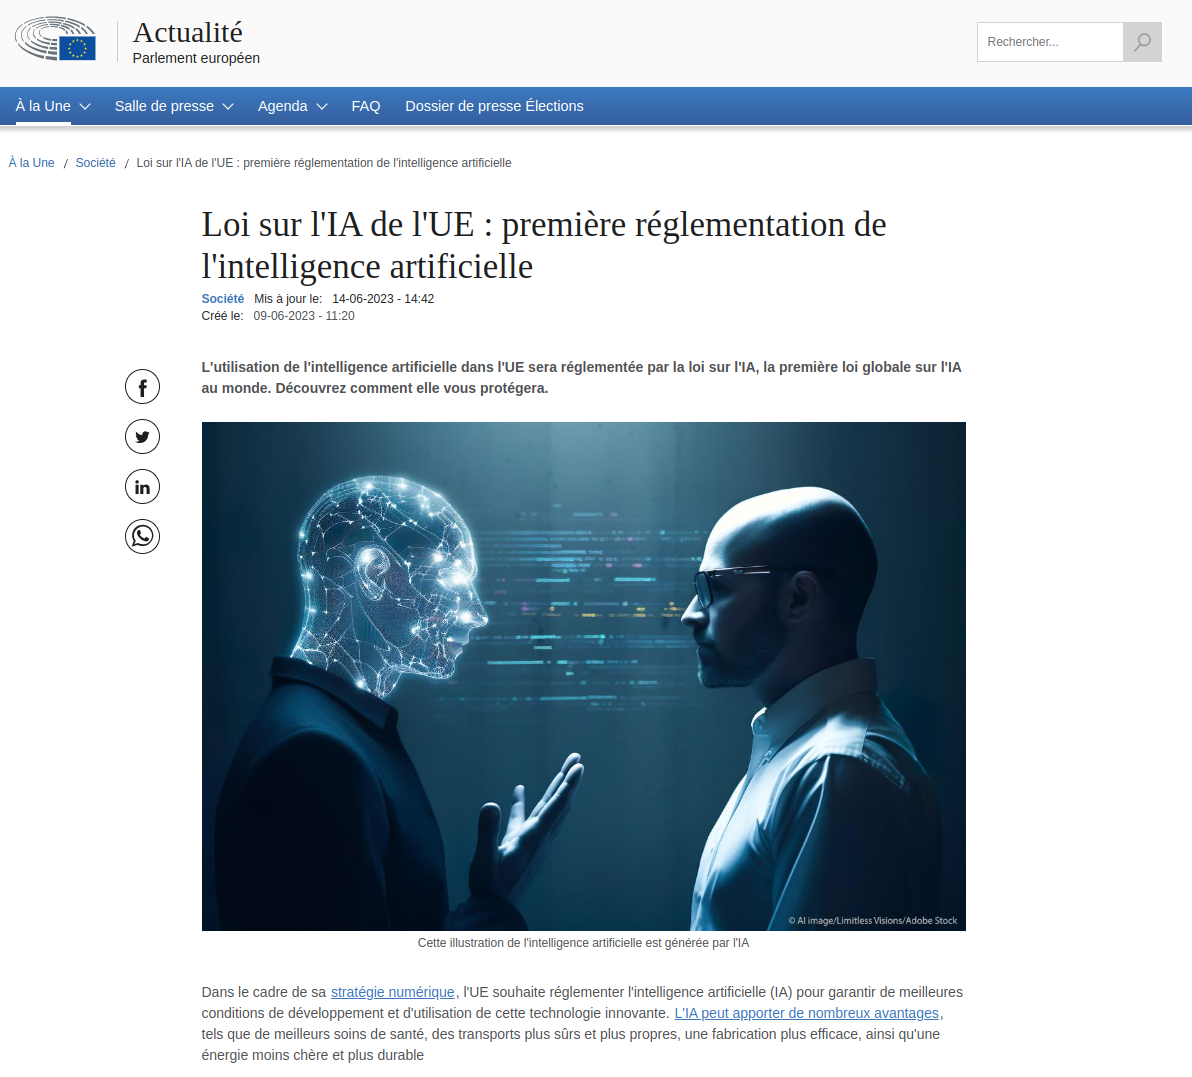
\includegraphics[width=0.90\textwidth]{04_Axe1_IAG/Images/AI-ACT.png}
\end{columns}
\end{frame}
